\documentclass[crop,dvisvgm,border=4pt]{standalone}

\usepackage{amsmath,amssymb}
  \usepackage{CJKutf8}
  \newcommand{\llbracket}{[\![}
  \newcommand{\rrbracket}{]\!]}
  \usepackage{tikz-cd}
  \usetikzlibrary{arrows.meta,backgrounds,calc,decorations.pathreplacing,fit,positioning,shapes.geometric}
  \newcommand{\pbcorner}{\vcenter{\hbox{\tikz[scale=.22]{\draw[line width=.55pt] (0,1)--(0,0)--(1,0);}}}}

\begin{document}
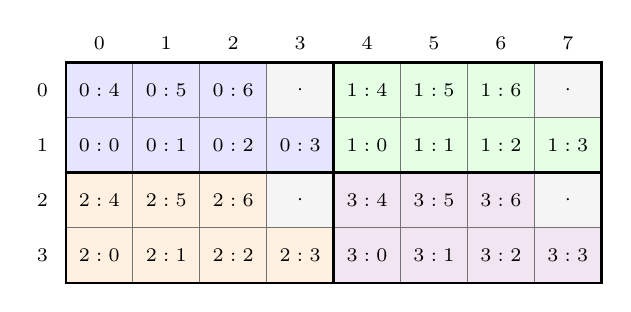
\begin{tikzpicture}[x=.85cm,y=.7cm,font=\scriptsize]
\fill[blue!10] (0,2) rectangle (4,4);
\fill[green!10] (4,2) rectangle (8,4);
\fill[orange!12] (0,0) rectangle (4,2);
\fill[violet!10] (4,0) rectangle (8,2);
\foreach \x/\y/\s in {0/2/0,4/2/1,0/0/2,4/0/3} {
  \fill[black!4] ({\x+3},{\y+1}) rectangle ({\x+4},{\y+2});
  \foreach \i in {0,...,6} {
    \node at ({\x+mod(\i,4)+.5},{\y+floor(\i/4)+.5}) {$\s:\i$};
  }
  \node at ({\x+3.5},{\y+1.5}) {$\cdot$};
}
\draw[step=1,black!55] (0,0) grid (8,4);
\draw[line width=.9pt] (0,0) rectangle (8,4);
\draw[line width=.9pt] (4,0) -- (4,4);
\draw[line width=.9pt] (0,2) -- (8,2);
\foreach \i in {0,...,7} {\node at ({\i+.5},4.35) {$\i$};}
\foreach \i in {0,...,3} {\node at (-.35,{3.5-\i}) {$\i$};}
\end{tikzpicture}
\end{document}
